\subsection{B.1 - \emph{Recozimento}}
O programa desenvolvido para essa simulação está abaixo: 

\begin{marginfigure}
    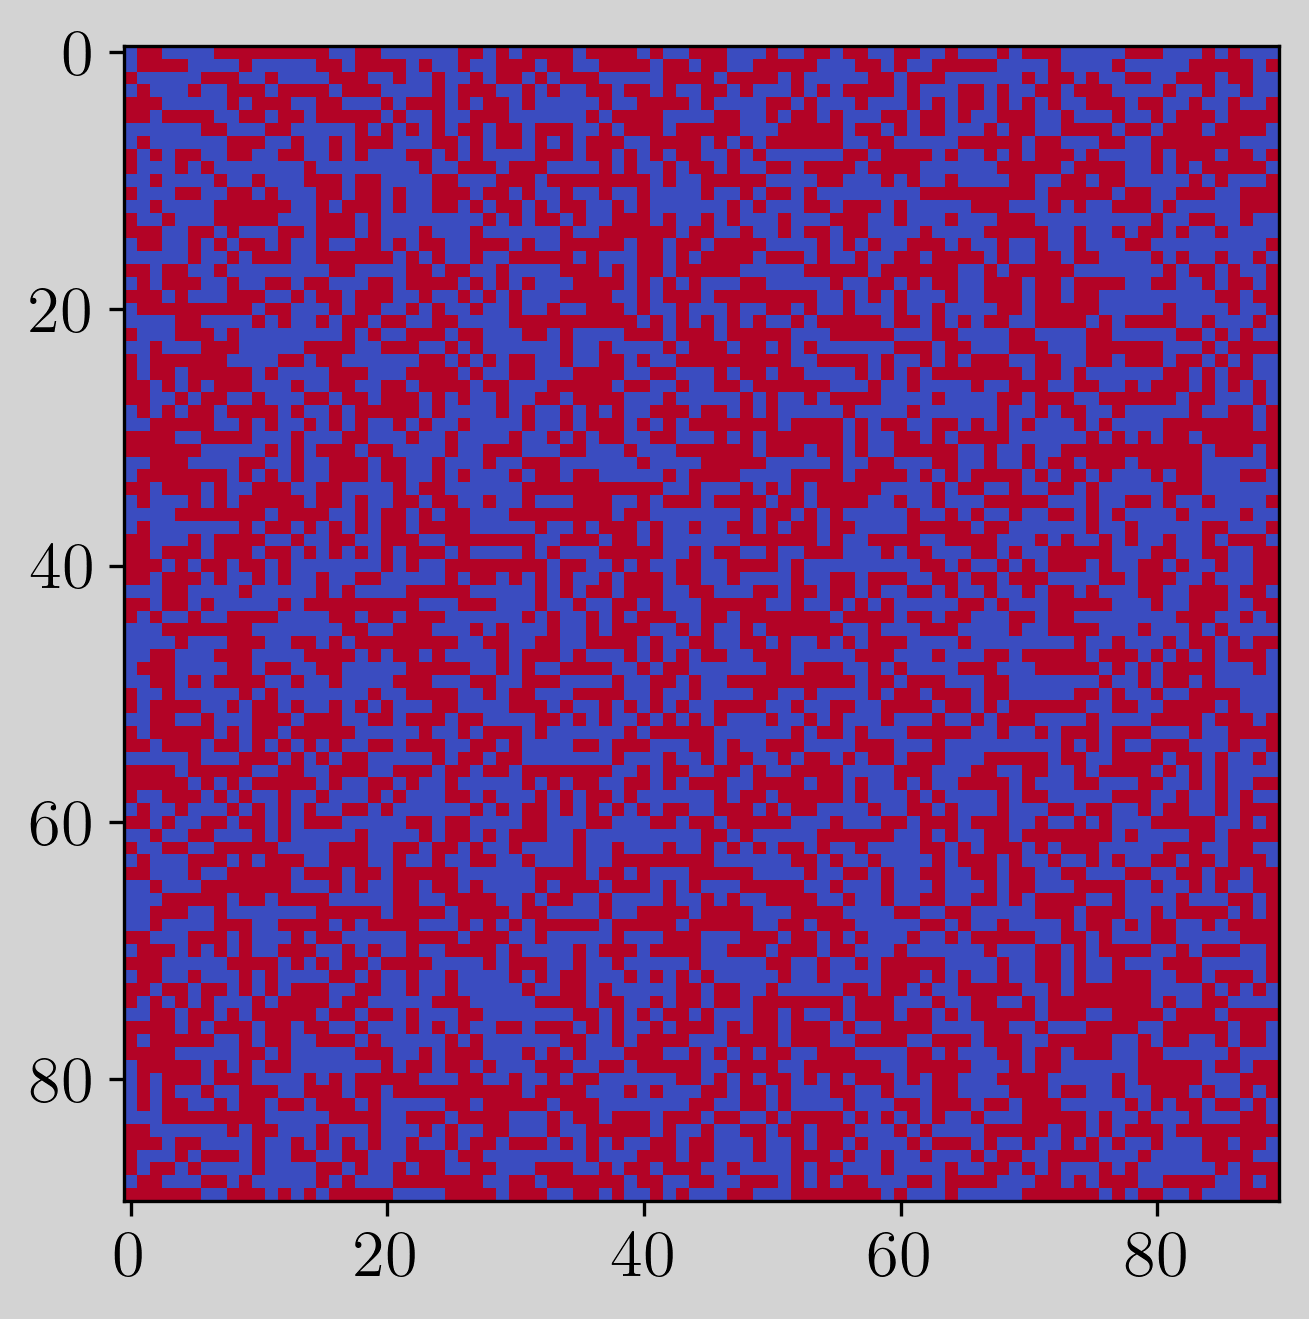
\includegraphics[width=0.8\linewidth]{graficos/tarefa-2/graf-tarefa-B1-conf-inicial.png}
    \caption{Configuração inicial da simulação. $\beta = 1/2$ }
    \label{fig:b1_conf_inicial}
\end{marginfigure}


\begin{minted}{fortran}
    !       Tarefa B - Recozimento e quenching
    implicit real(j-j, m-m)
    parameter(L = 100)
    dimension exps(-4:4)
    byte lattice(1:L, 1:L)

    ! periodic boundary conditions
    dimension ipbc(0:L+1)

    L_real = 90

    do i = 1, L_real
        ipbc(i) = i
    end do  
    ipbc(0) = L_real
    ipbc(L_real+1) = 1

    N = L_real * L_real

    mag = 0.0d0

    call srand(351324)

    call initialize_random_lattice(lattice,  L_real, L_real)

    open(1, file="saidas/tarefa-2/saida-tarefa-B1-conf-inicial.dat")
    open(2, file="saidas/tarefa-2/saida-tarefa-B1-conf-final.dat")
    open(3, file="saidas/tarefa-2/saida-tarefa-B1-mag-eng.dat")

    call write_lattice(lattice, L_real, 1) 
    call total_magnetization(lattice, mag, L_real)

    ! initial energy
    E = H_0(lattice, ipbc, L_real)

    dbeta = 0.001
    ! monte carlo dynamics
    do i = 1, 3000
        beta = i * dbeta
        call define_exponentials(exps, beta)
        do k = 1 , N
              call flip_spin(lattice,ipbc,exps,E,mag,L_real)
        end do   
        write(3, *) i, mag, E/N
    end do
    call write_lattice(lattice, L_real, 2) 
    close(1)
    close(2)
    close(3)
    end
\end{minted}


Fazendo evolução da temperatura de forma lenta, com $\Delta \beta = 0.001$ temos o processo de recozimento. 
Partimo do sistema desordenado, com temperatura infinita e a cada passo de Monte Carlo provocamos uma variação
de temperatura $\Delta \beta$. A figura (\ref{fig:b1_conf_inicial}) mostra a configuração inicial do sistema de spins.



Estamos interessados em observar a energia média por spin. Pelo gráfico 
abaixo(\ref{fig:tarefa_b1_graf_energia}) nota-se que a energia média parte de zero, pois o sistema 
está completamente desordenado, e decresce até atingir  a energia limite em $-2$. 

\begin{figure}
    \centering
    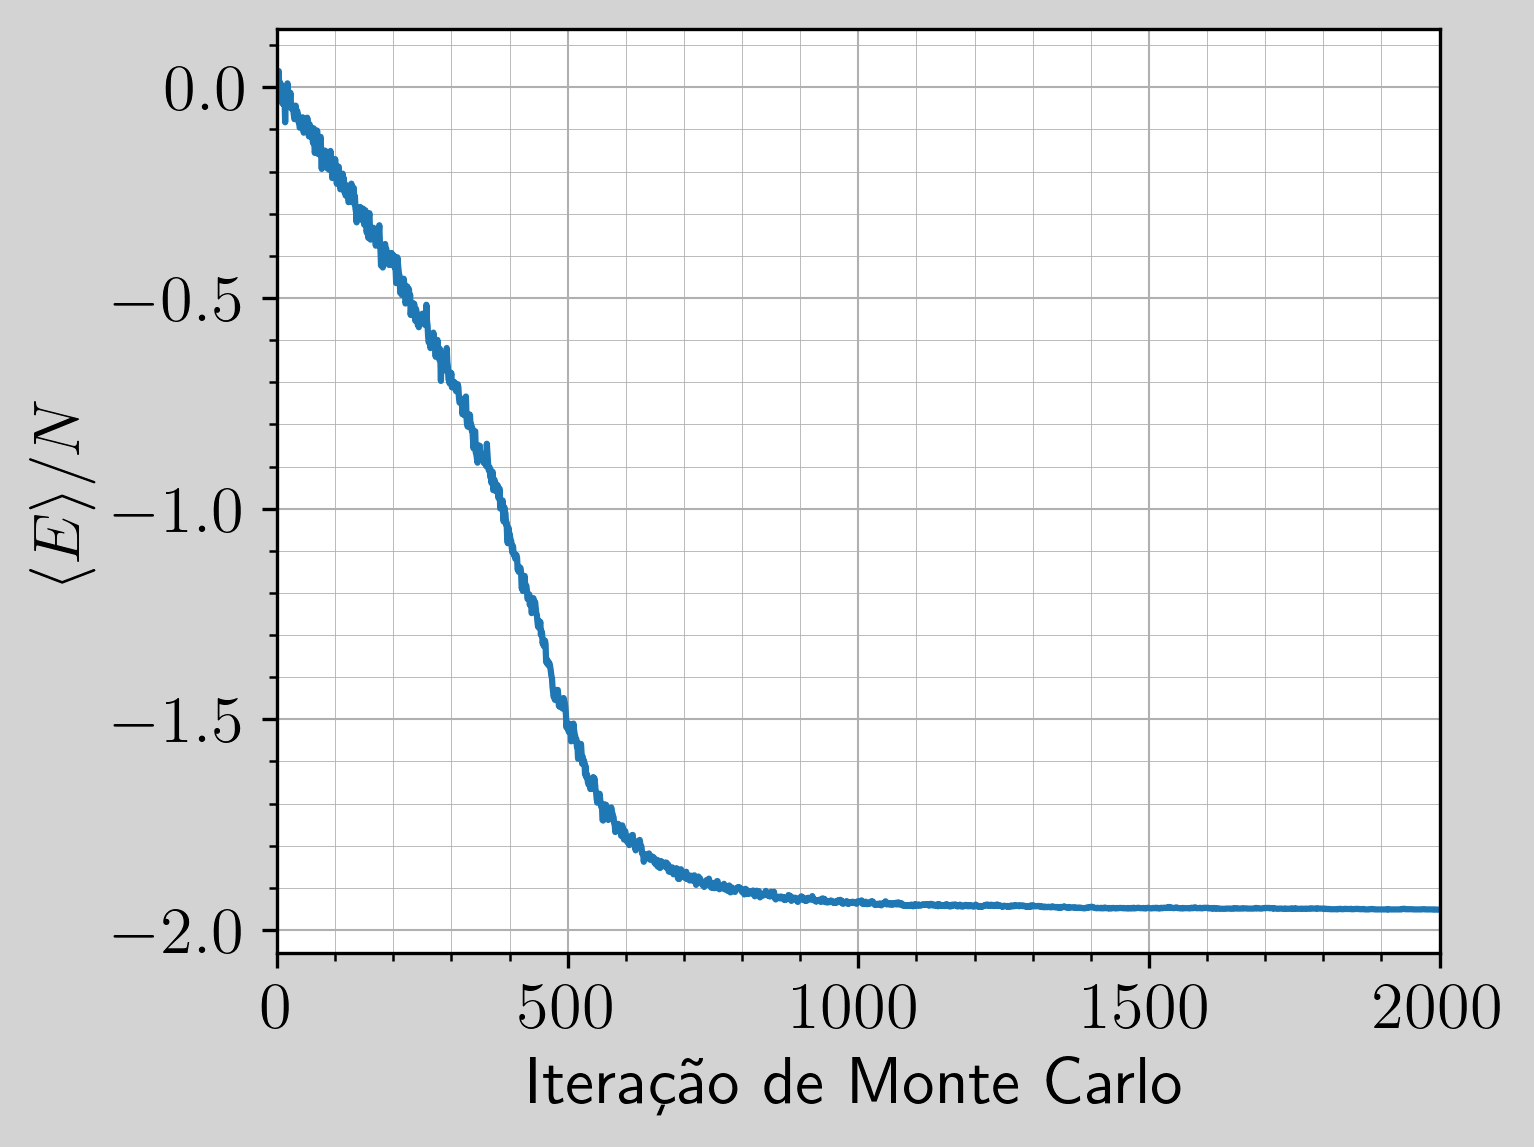
\includegraphics[width=0.6\linewidth]{graficos/tarefa-2/graf-tarefa-B1-mag-eng.png}
    \caption{Energia média de spin por iterações de Monte Carlo.}
    \label{fig:tarefa_b1_graf_energia}
\end{figure}


Além disso, temos a configuração final dos spins do sistema bidimensional(\ref{fig:b1_conf_final}). 
Há uma faixa de magnetização na malha, a presença dela deve estar associada ao número de iterações de Monte Carlo feita
utilizado na simulação ($3000$ passos) que não foi o bastante para o sistema ficar todo alinhado. 

\begin{marginfigure}
    \centering
    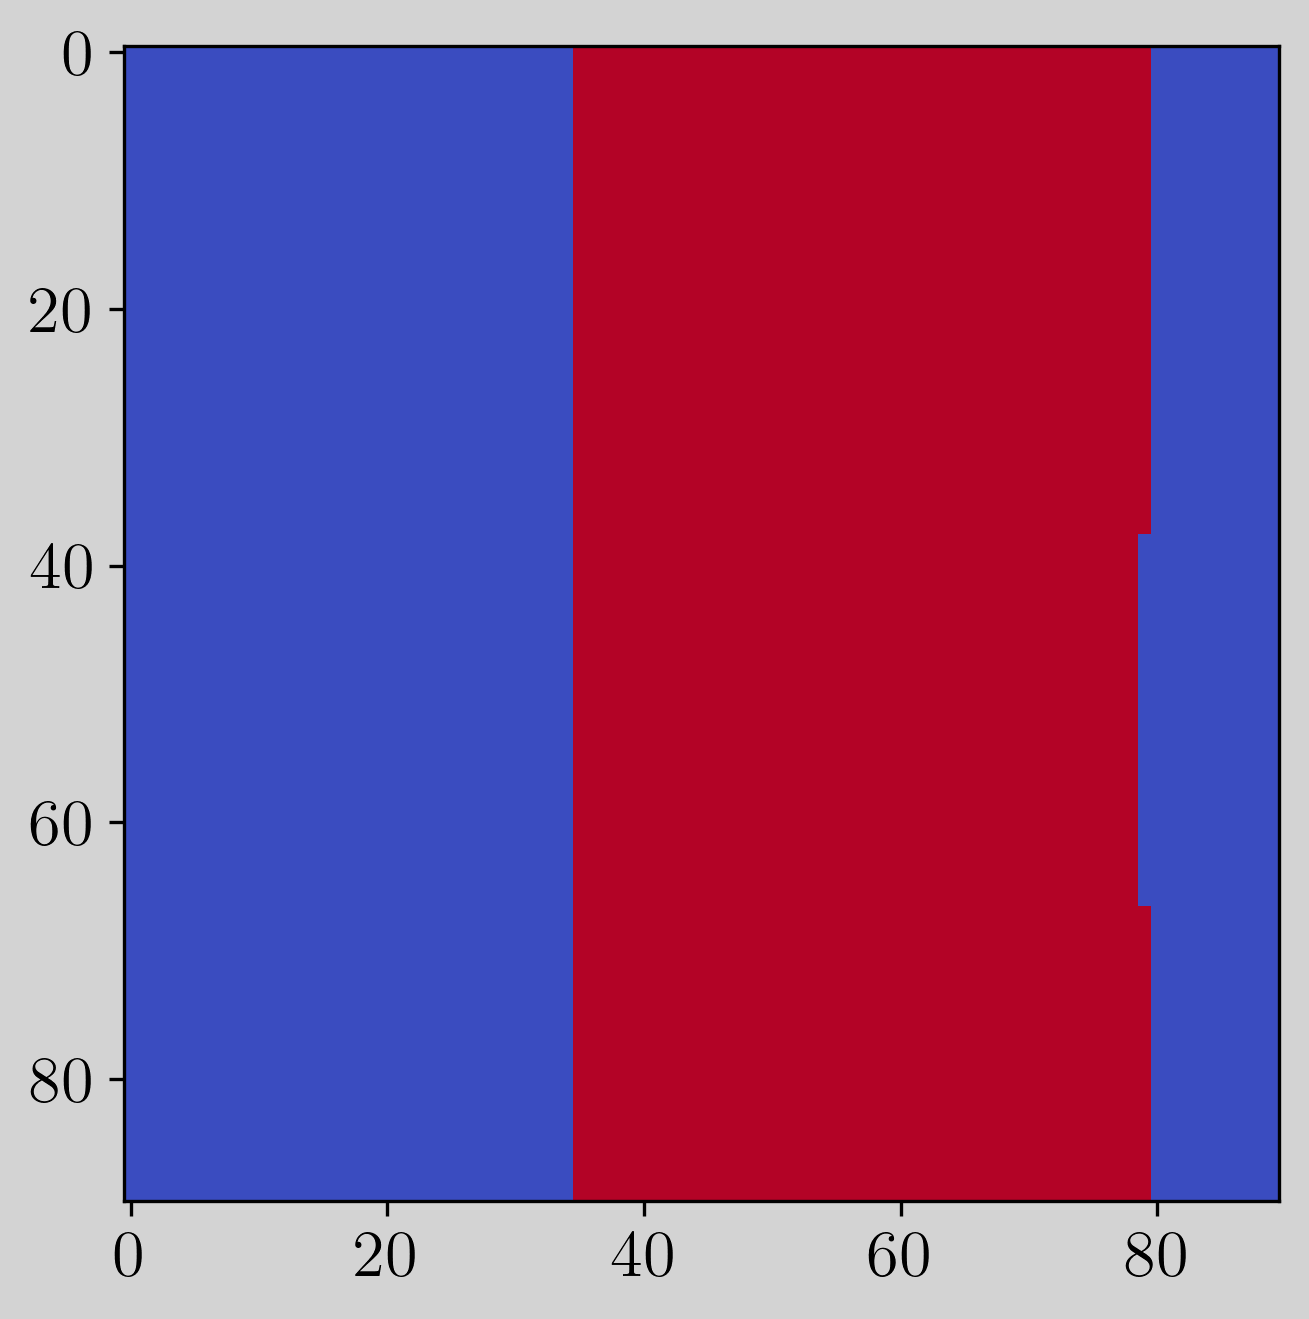
\includegraphics[width=0.8\linewidth]{graficos/tarefa-2/graf-tarefa-B1-conf-final.png}
    \caption{Configuração final da malha 2D após dinâmica de recozimento.}
    \label{fig:b1_conf_final}
\end{marginfigure}

% \clearpage
\subsection{B.2 - \emph{Tempera}}
O código dessa simulação é quase idêntico ao da tarefa anterior e está compilado abaixo: 

\begin{minted}{fortran}
        implicit real(j-j, m-m)
        parameter(L = 100)
        dimension exps(-4:4)
        byte lattice(1:L, 1:L)

        ! periodic boundary conditions
        dimension ipbc(0:L+1)
    
        L_real = 90
        
        do i = 1, L_real
            ipbc(i) = i
        end do

        ipbc(0) = L_real
        ipbc(L_real+1) = 1

        N = L_real * L_real

        mag = 0.0d0
        
        call srand(96312)
        call initialize_random_lattice(lattice,  L_real, L_real)
        
        open(1, file="saidas/tarefa-2/saida-tarefa-B2-conf-inicial.dat")
        open(2, file="saidas/tarefa-2/saida-tarefa-B2-conf-final.dat")
        open(3, file="saidas/tarefa-2/saida-tarefa-B2-mag-eng.dat")
        
        call write_lattice(lattice, L_real, 1) 

        call total_magnetization(lattice, mag, L_real)
         
        ! initial energy
        E = H_0(lattice, ipbc, L_real)


        dbeta = 0.001
        write(3, *) 0, mag, E/N
        ! monte carlo dynamics
        beta = 3

        call define_exponentials(exps, beta)
        do i = 1, 3000
            do k = 1 , N
                  call flip_spin(lattice,ipbc,exps,E,mag,L_real)
            end do   
            write(3, *) i, mag, E/N
        end do
        call write_lattice(lattice, L_real, 2) 
        close(1)
        close(2)
        close(3)
        end
\end{minted}

Nessa simulação partimos da mesma configuração inicial que a anterior 
e  variamos o $\beta$ de maneira brusca e o sistema pode não atingir o equiblirio. Foi utilizada 
uma malha de tamanho $L= 90$ para essa simulação e mesmo número de passos. 

\begin{figure}
    \centering
    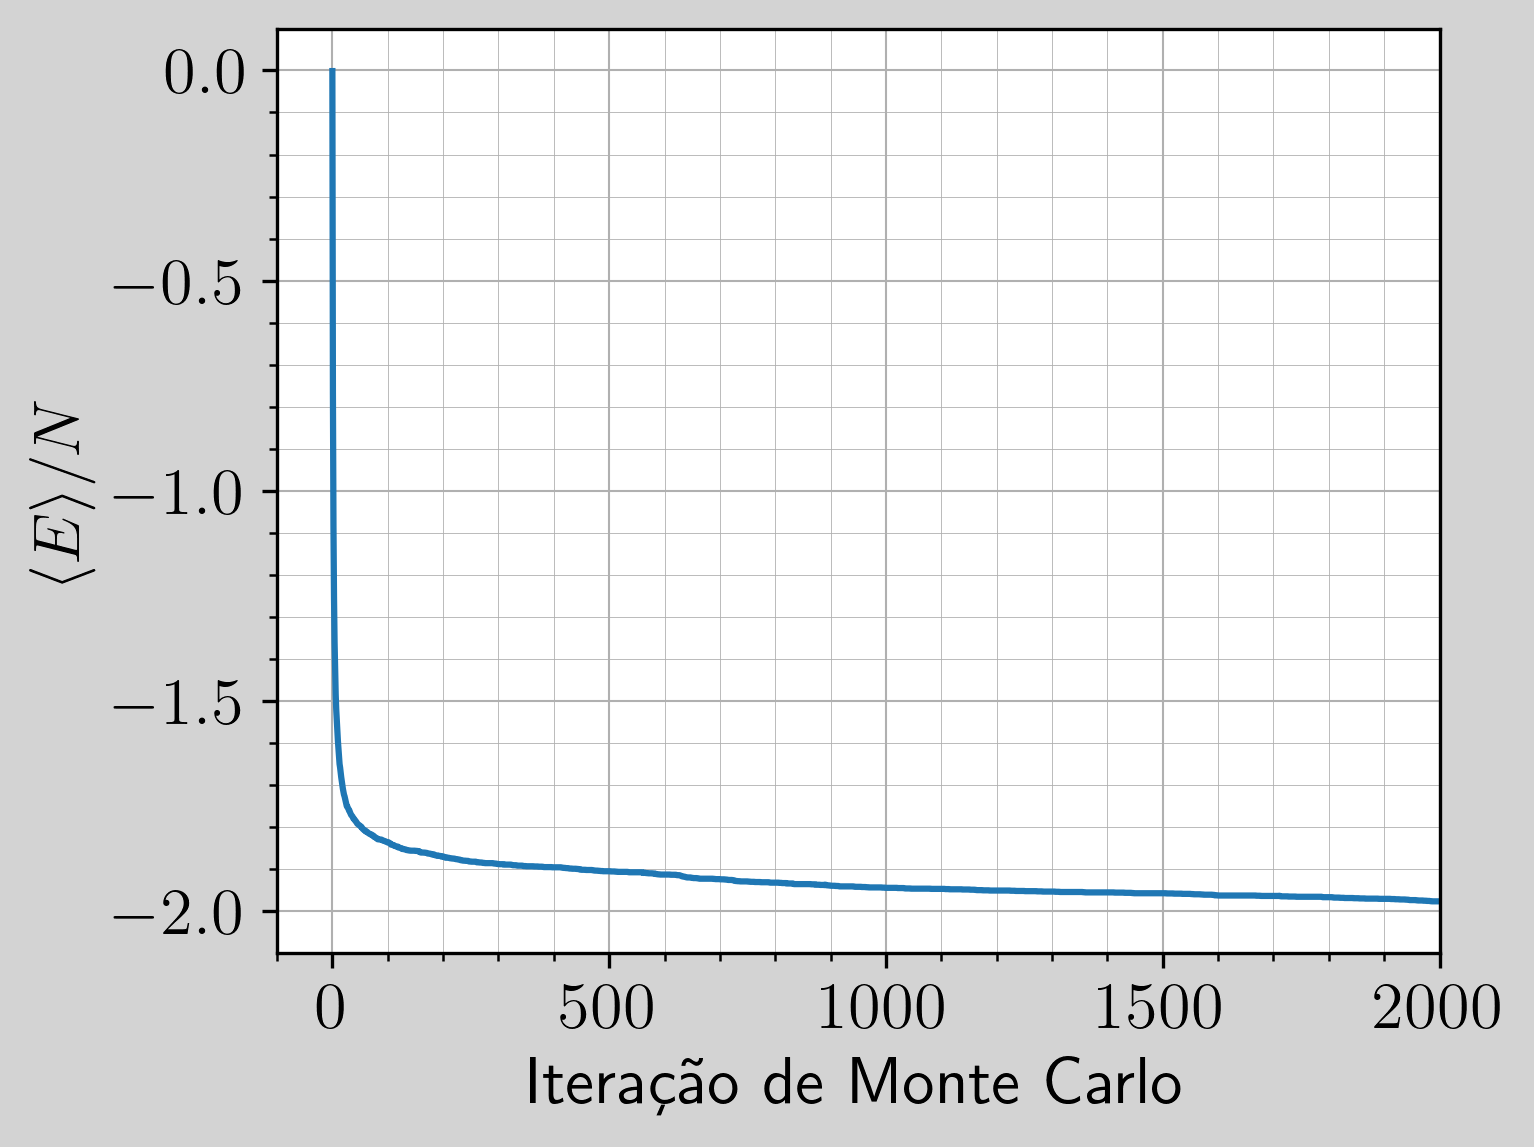
\includegraphics[width=0.6\linewidth]{graficos/tarefa-2/graf-tarefa-B2-mag-eng.png}
    \caption{Energia média de spin por iterações de Monte Carlo.}
\end{figure}

Nota-se que a energia média decaí muito mais rapidamente que no caso anterior(\ref{fig:tarefa_b1_graf_energia})
e a configuração final consegue atingir o equiblirio(\ref{fig:b2_conf_final}). Diferentemente do processo anterior, na têmpera 
os spins vizinhos conseguem se alinhar no tempo de Monte Carlo utilizado na simulação.

\begin{marginfigure}
    \centering
    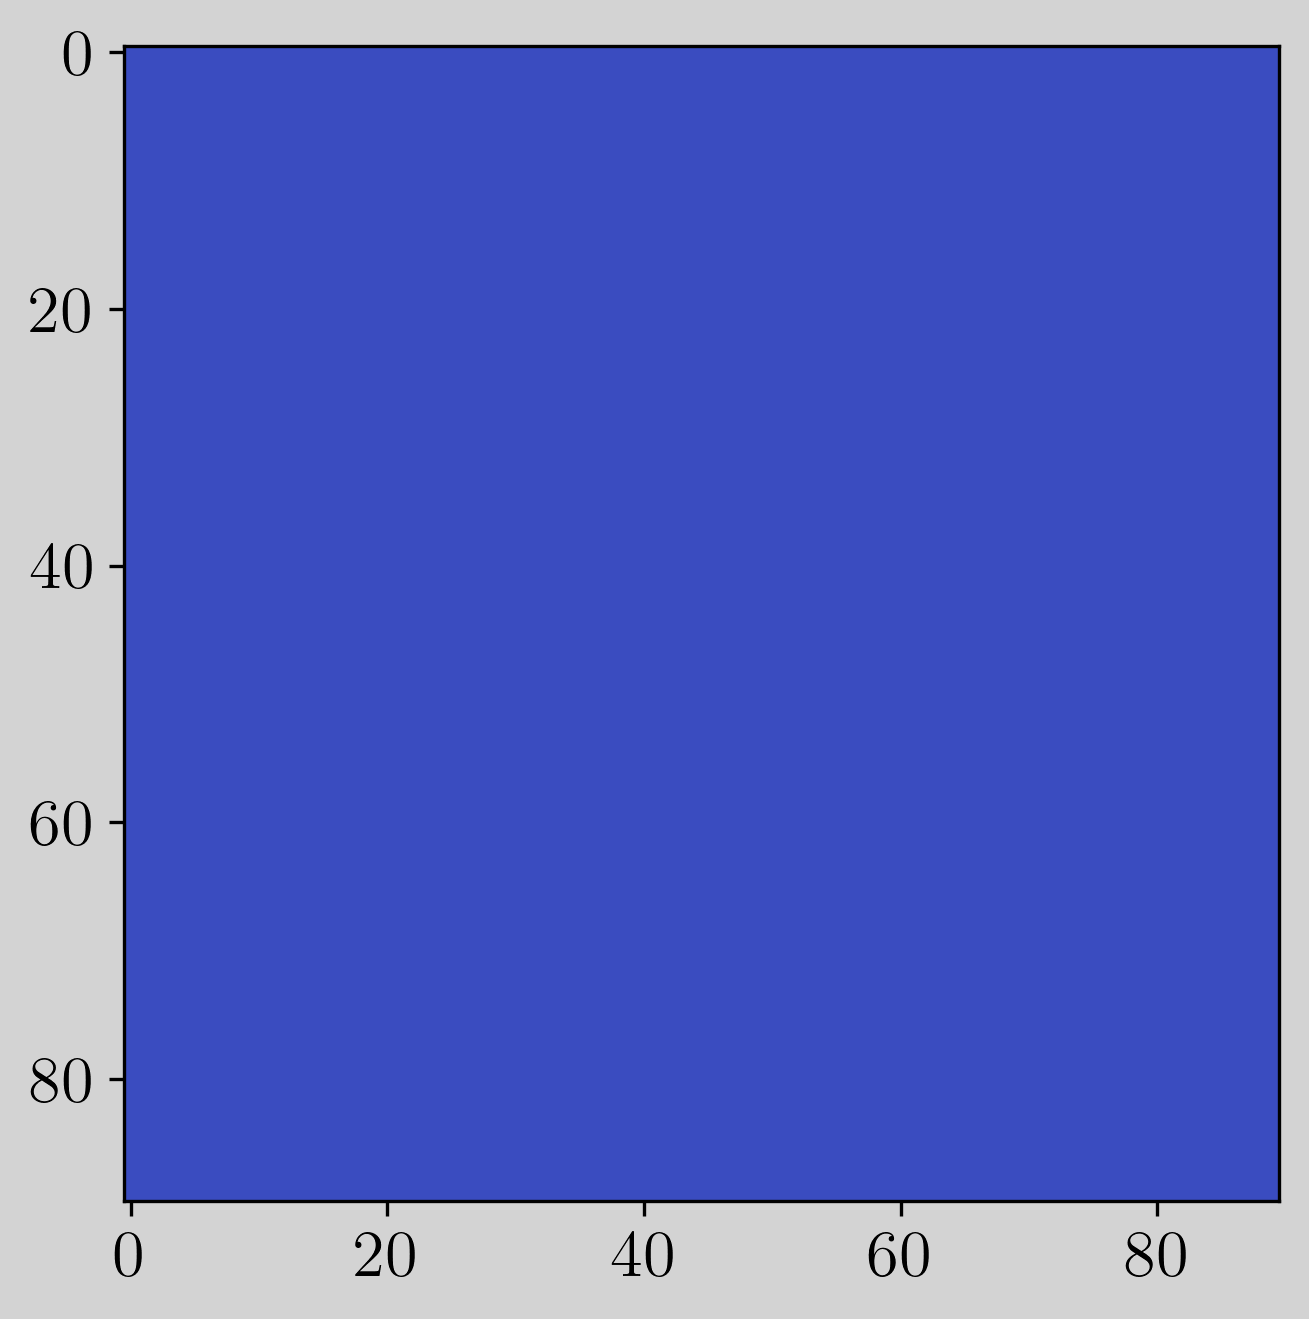
\includegraphics[width=0.8\linewidth]{graficos/tarefa-2/graf-tarefa-B2-conf-final.png}
    \caption{Configuração final para rede de spins na dinâmica de têmpera.}
    \label{fig:b2_conf_final}
\end{marginfigure}